% !TEX encoding = UTF-8
% !TEX TS-program = pdflatex
% !TEX root = ../apprendimento_automatico.tex
% !TEX spellcheck = it-IT
\section{Lezione 7 - Alberi di decisione}\label{lezione-7---alberi-di-decisione}

In molte situazioni del mondo reale non è sufficiente apprendere
funzioni booleane con ingressi binari (quello che si fa con il concept
learning).

Gli alberi di decisione funzionano bene con:

\begin{itemize}
\item
  Istanze rappresentate da coppie attributo-valore
\item
  Funzioni target con valori di output discreti (più di due valori),
  come il riconoscimento della categoria di una pagina web
\item
  Concetti descritti da disgiunzioni di funzioni booleane
\item
  Esempi di apprendimento che possono contenere errori e/o valori
  mancanti (es: diagnosi medica senza alcuni esami).
\end{itemize}

Gli algoritmi che lavorano su alberi di decisione sono molto efficienti
ed è per questo che vengono utilizzati in applicazioni pratiche.

\subsection{È il giorno giusto per giocare atennis?}\label{uxe8-il-giorno-giusto-per-giocare-a-tennis}

Dati:

\begin{figure}[htbp]
\centering
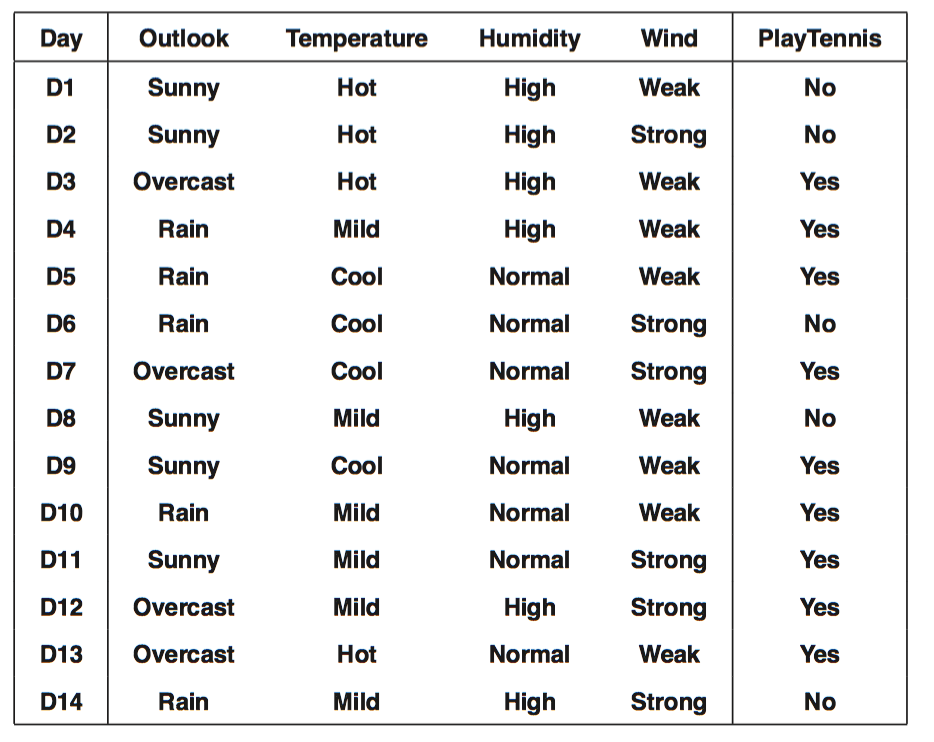
\includegraphics[width=0.5\textwidth]{./notes/immagini/l7-tabella.png}
\caption{Dataset per il tennis}
\end{figure}
\FloatBarrier
Albero:

\begin{figure}[htbp]
\centering
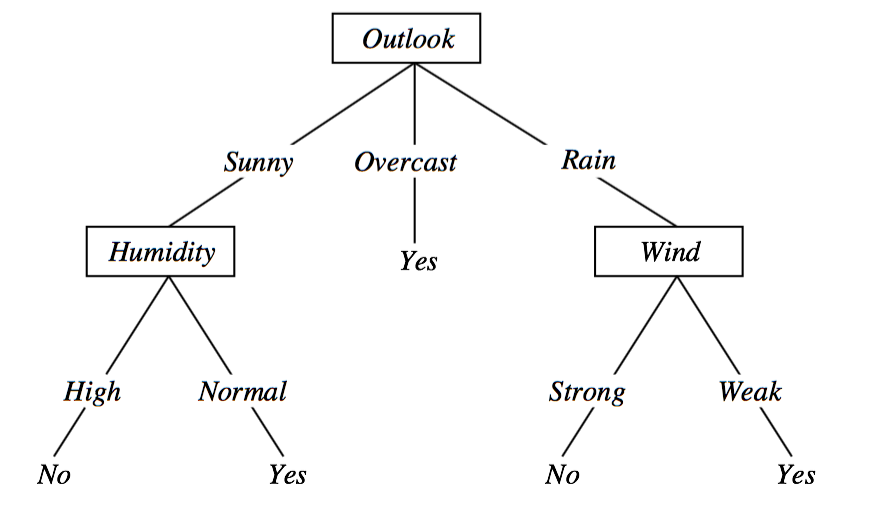
\includegraphics[width=0.5\textwidth]{./notes/immagini/l7-albero.png}
\caption{Albero di decisione per il tennis}
\end{figure}
\FloatBarrier

Come si può notare, nell'albero ogni nodo corrisponde ad un attributo e
l'arco tra un nodo e l'altro corrisponde uno dei possibili valori,
mentre le foglie dell'albero forniscono una classificazione.

Per classificare un'istanza si parte dalla radice e si scende verso le
foglie, secondo quanto specificato dai test sugli attributi definiti dai
nodi dell'albero.

Se si raggiunge una foglia l'etichetta ad essa associata rappresenta la
classificazione.

Dato un albero di decisione, questo corrisponde ad una
\textbf{disgiunzione di congiunzioni}.

Lo stesso albero può essere infatti rappresentato come:

\begin{verbatim}
(Outlook = Sunny and Humidity = Normal) 
            or 
    (Outlook = Overcast)
            or
(Outlook = Rain and Wind = Weak) 
\end{verbatim}

\subsection{ID3 - Apprendimento su un albero}\label{id3---apprendimento-su-un-albero}

L'algoritmo di apprendimento che costruisce l'albero di decisione
tramite una procedura top down in stile divide et impera.

La costruzione inizia con la domanda ``\emph{Quale
attributo dovrebbe essere testato alla radice dell'albero?}''. Per
scegliere l'attributo vengono valutati tutti i possibili candidati
utilizzando un test statistico per valutare quanto bene il singolo
attributo classifica il training set.

Viene selezionato il miglior attributo e utilizzato come test alla
radice dell'albero. Vengono poi creati tanti figli quanti sono i
possibili valori dell'attributo e gli esempi del training set vengono
partizionati tra i vari figli, in modo che il loro valore per
quell'attributo corrisponda con il valore del nodo.

Questo processo viene ripetuto per ognuno dei nodi creati fino a che
non vengono esaminati tutti gli esempi.

Più formalmente, dato un training set \emph{Tr} e un insieme di
attributi \emph{A}, algoritmo è definito come:

\begin{enumerate}
\item
  Crea il nodo radice, copia in \emph{T} gli esempi di \emph{Tr} e
  inserisce tutti gli attributi in \emph{A}.
\item
  Se gli esempi in \emph{T} sono tutti delle stessa classe, ritorna
  l'albero con un solo nodo e etichetta uguale alla classe.
\item
  Se \emph{A} è vuoto, ritorna l'albero con un solo nodo e come
  etichetta la classe di maggioranza in \emph{T}.
\item
  Altrimenti, si sceglie l'attributo \emph{a} tra gli attributi presenti
  in \emph{A} (il migliore) e si partiziona \emph{T} secondo i possibili
  valori che l'attributo \emph{a} può assumere: $T_a = val_1, \ldots,  T_a = val_n$:
 \begin{enumerate}
  \item
    Per ogni $T_a = val_i$, se è vuoto crea una foglia con
    l'etichetta della classe più frequente in \emph{T}, altrimenti crea un
    sotto-albero con l'algoritmo ID3 con $T_a = val_i$ e \emph{A -\{}\textit{a}\emph{\}}.
  \end{enumerate}
\item
  Ritorna \emph{T}.
\end{enumerate}

Quando una partizione risulta vuota, vuol dire che non esistono esempi
nel training set per i quali il valore dell'attributo selezionato è
uguale a quel dato valore, quindi viene assegnato alla foglia il valore più comune all'interno del training set.

\subsubsection{Esempio sui dati del tennis}\label{esempio-sui-dati-del-tennis}

\begin{verbatim}
T = {D1, ..., D14}
A = {Outlook, Temperature, Humidity, Wind}

a = Outlook

                   (Outlook)
               /       |       \
            sunny    overcast   rain
            /          |          \
(T_Overlook = Sunny
A = Temp, Hum, Wind})
\end{verbatim}

Al secondo passo mi ritrovo scelgo \texttt{a\ =\ Humidity}, ottenendo:

\begin{verbatim}
                   (Outlook)
               /       |       \
            sunny    overcast   rain
            /          |          \
       (Humidity)
       /        \
    High        Normal
    /               \
   No               Si
\end{verbatim}

In questo caso i figli vengono marcati con un valore nel
caso in cui tutti gli esempi della partizione hanno lo stesso valore
target.

Si prosegue finché l'albero non è completo

\subsubsection{Alla ricerca dell'attributo ottimo}\label{alla-ricerca-dellattributo-ottimo}

Nell'esempio precedente è stato scelto un attributo a caso, ma nel caso
pratico questo non conviene.

Come viene scelto l'ottimo dipende da algoritmo ad algoritmo, nel caso
di ID3 vengono utilizzati i concetti di \emph{entropia} e \emph{guadagno
entropico}.

$$
E(S) = -p-log_2(p_-) -p+log_2(p_+)
$$

Dove $p_-$ e $p_+$ rappresentano la proporzione degli esempi della di una
classe e dell'altra (si assume che ci siano solo due classi) all'interno
dell'insieme \textit{S}.

L'entropia misura il grado di impurità dell'insieme degli esempi.

Nel caso ci siano più valori l'entropia si calcola come

$$
E(S) = - \sum_v p_vlog_2(p_v)
$$

ID3 sceglie come attributo \emph{a}, quello che massimizza il guadagno
entropico.

$$
G(S,a) = E(S) - \sum_{v \in V(a)} \frac{|S_{a = v}|}{|S|} E(S_{a=v})
$$

Il guadagno misura la riduzione aspettata dell'entropia nel partizionare
i dati utilizzando l'attributo \emph{a}.

L'entropia attesa è descritta dal secondo termine ed è semplicemente la
sommatoria delle entropie di tutti i sottoinsiemi di \emph{S}, pesata
secondo il numero di esempi che appartengono al sottoinsieme di
\emph{S}.

\textbf{Problema}: L'utilizzo del guadagno entropico favorisce troppo
gli attributi che possono assumere tanti valori diversi, ad esempio
l'attributo \emph{Data}. 
Scegliere un attributo di questo tipo porta ad ottenere tante partizioni, ognuna di pochi
elementi e che non forniscono informazioni utili.

Per evitare ciò al posto del guadagno si può utilizzare:

$$
GainRatio(S, a) = \frac{G(S, a)}{SI(S,a)}
$$

Dove \emph{SI} rappresenta la \emph{split information}, un valore che
misura quanti e quanto uniformi sono i sottoinsiemi generati
dall'attributo \emph{a} a partire dall'insieme \emph{S}.

$$
SI(S,a) = - \sum_{v \in V(a)}\frac{|S_{a = v}|}{|S|} log_2(\frac{|S_{a = v}|}{|S|})
$$

E corrisponde all'entropia di \emph{S} dati i possibili valori di
\emph{a}.

\emph{GainRatio} non risolve tutti i problemi, infatti può succedere che
attributi significativi e che possono assumere tanti valori vengano
svantaggiati rispetto al altri.

L'idea più comunque è quella di calcolare il guadagno \emph{G} per ogni
attributo e fare la media dei valori trovati, per poi andare a
scegliere tra gli attributi con \emph{G} sopra la media,
l'attributo che ha \emph{GainRatio} maggiore.
